\subsection{Optimizations for Leiden algorithm}
\label{sec:leiden}

We extend our optimizations for the Louvain algorithm \cite{sahu2023gvelouvain}, to the Leiden algorithm. In detail, we employ an \textit{asynchronous} implementation of the \textit{Leiden} algorithm, where threads operate independently on distinct sections of the graph. This facilitates quicker convergence but introduces variability into the final result \cite{com-blondel08}. To perform computations efficiently, we pre-allocate a dedicated hashtable per thread. These hashtables serve two primary purposes: they keep track of the delta-modularity associated with moving to each community connected to a vertex during the local-moving/refinement phases, and they record the total edge weight between super-vertices in the aggregation phase of the algorithm.

Our optimizations encompass several strategies, including utilizing OpenMP's \textit{dynamic} loop scheduling, capping the number of iterations per pass at $20$, employing a tolerance drop rate of $10$ (threshold scaling), initiating with a tolerance of $0.01$, using an aggregation tolerance of $0.8$ to avoid performing aggregations of minimal utility, implementing flag-based vertex pruning (instead of a queue-based one \cite{nguyenleiden}), utilizing parallel prefix sum, and using preallocated Compressed Sparse Row (CSR) data structures for identifying community vertices and storing the super-vertex graph during aggregation. Additionally, we employ fast collision-free per-thread hashtables, well separated in their memory addresses.

We attempt two variants of the \textit{Leiden} algorithm. One uses a \textit{greedy refinement phase} where vertices greedily optimize for delta-modularity (within their community bounds), while the other uses a \textit{random-greedy refinement phase} (using a fast \textit{xorshift32} random number generator), where the likelihood of selection of a community to move to (by a vertex) is proportional to its delta-modularity. Our experiments show the \textit{greedy variant} performs the best on average, both in terms of runtime and modularity. We also try medium and heavy variants which disable threshold scaling and aggregation tolerance, however do not find them to perform well overall. On \textit{europe\_osm} graph, our parallel Greedy-Leiden (which we from here on refer to simply as Leiden) runs $3\times$ faster than Nguyen \cite{nguyenleiden}.

\begin{figure*}[hbtp]
  \centering
  \subfigure{
    \label{fig:leiden-opt--all}
    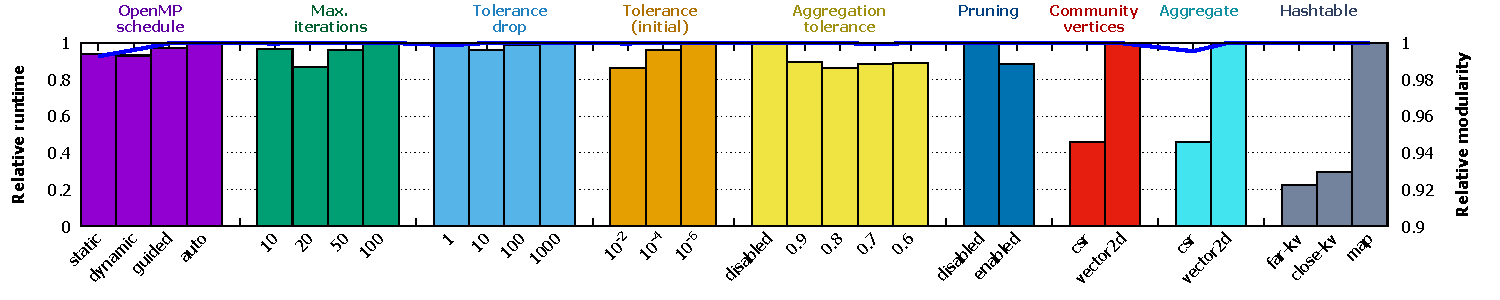
\includegraphics[width=0.98\linewidth]{out/leiden-opt.pdf}
  } \\[-2ex]
  \caption{Impact of various parameter controls and optimizations on the runtime and result quality (modularity) of the \Lou{} algorithm. We show the impact of each optimization upon the relative runtime on the left Y-axis, and upon the relative modularity on the right Y-axis.}
  \label{fig:leiden-opt}
\end{figure*}


%% Also include algorithm for counting disconnected communities
Counting of disconnected communities is taking much longer (>30min). Current algorithm obtains the vertices belonging to each community (ID) and checks if all vertices within the community are reachable (using BFS or DFS from one vertex in each community), while avoiding to go to any other adjacent community.

Now i am trying to optimize the method for examining disconnected communities.
The base algorithm is as follows:
- Find the size of each community
- Pick one vertex from each community
- Traverse from that vertex within the community
- If all vertices within the community could not be reached, we know its disconnected

I try four different variations of this algorithm which differ in whether we use:
- Parallel DFS or BFS
- Per-thread or shared "visited" flags (shared flags is called light DFS/BFS)
(If it is shared, each thread should scan all vertices but only process that community which belongs to it -> this is determined by community-id)

It appears BFS traversal with a shared flag vector is the fastest. This is not a heuristic algorithm, so all algorithms return the same result.


%% Additional notes on Leiden algorithm
I fixed the bug that caused leiden algorithm to fail if finding communities on road networks and kmer graphs. The issue was forgetting to reset the affected vertices flags before running the refinement phase.




\subsection{Our optimized Leiden implementation}

We now explain the implementation of GVE-Leiden in Algorithms \ref{alg:leiden}, \ref{alg:leidenlm}, and \ref{alg:leidenag}. A flow diagram illustrating the first pass of GVE-Leiden is shown in Figure \ref{fig:leiden-pass}.


%% Our implementation of Leiden algorithm
On europe\_osm our algorithm runs in 23s (~3x speedup wrt Fabien). I also try medium and heavy variants which disable threshold scaling and aggregation tolerance. Results show that louvain is on average 1.4x faster than leiden (optimized greedy variation). In terms of modularity, leiden (greedy variant) obtains slightly higher modularity than louvain. Leiden however improves upon louvain by obtaining 20x fewer disconnected communities (at 1.4x runtime cost).


%% Yet again on Leiden algorithm
I tried two variations of Leiden algorithm (like before):
- Greedy Leiden: Where the refinement phase is greedy, just like local-moving phase
- Random Leiden: Where refinement phase is proportionally random to delta-modularity, as proposed by Traag et al.
(For random leiden, i use xorshift32 random number generator, C++ default RNG too slow)

Further i try 3 different variations of Greedy/Random Leiden:
- Normal: Uses same paramter config as our optimized Louvain (tolerance=$10^-2$, 20 max iterations, 5 max passes)
- Medium: Uses lower start tolerance of $10^-6$, 100 max iterations, 100 max passes
- Heavy: Uses even lower start tolerance of $10^-10$, 100 max iterations, 100 max passes
(The idea is to see if my normal Leiden configs are good or not)

Please ignore road networks and k-mer protien graphs, as Leiden does not work there, will try to explain why so later.

Here are the observations:
- Greedy Leiden is faster than Random Leiden
- Medium/Heady variations generally dont do well, so my normal configs are good
- Louvain is genrally faster than Leiden

Louvain generally obtain communities of higher modularity than Leiden.
However, a large fraction of communities obtained by Louvain are disconnected.

Q> Why does Leiden have some disconnected communities still?
Q> Why does Leiden not work with road networks?
I think the answer for both questions has to do with parallelism. There is a race between threads to pick a suitable community. If the size of each community is large, this generally does not badly affect modularity. But with small community bounds (in refinement phase of Leiden) the race can lead to bad community memberships. I will try to come up a few solutions to this. This is not an issue with sequential, so Traag et al. dont observe this issue in their original paper.
https://www.nature.com/articles/s41598-019-41695-z




\subsubsection{Main step of GVE-Leiden}

The main step of GVE-Leiden (\texttt{louvian()} function) is outlined in Algorithm \ref{alg:leiden}. It encompasses initialization, the local-moving phase, and the aggregation phase. Here, the \texttt{leiden()} function takes the input graph $G$, and returns the community membership $C$ for each vertex. In line \ref{alg:leiden--initialization}, we first initialize the community membership $C$ of each vertex in $G$, and perform passes of the Louvain algorithm, limited to $MAX\_PASSES$ (lines \ref{alg:leiden--passes-begin}-\ref{alg:leiden--passes-end}). In each pass, we initialize the total edge weight of each vertex $K'$, the total edge weight of each community $\Sigma'$, and the community membership $C'$ of each vertex in the current graph $G'$ (line \ref{alg:leiden--reset-weights}); and mark all vertices as unprocessed (line \ref{alg:leiden--reset-affected}).

Next, in line \ref{alg:leiden--local-move}, we perform the local-moving phase by calling \texttt{leidenMove()} (Algorithm $\ref{alg:leidenlm}$), which optimizes community assignments. If the local-moving phase converged in a single iteration, global convergence is implied and we terminate the passes (line \ref{alg:leiden--globally-converged}). Further, if the drop is community count $|\Gamma|$ is too small, we have reached the point of diminishing returns, and thus stop at the current pass (line \ref{alg:leiden--aggregation-tolerance}).

In case convergence has not been achieved, we renumber communities (line \ref{alg:leiden--renumber}), update top-level community memberships $C$ with dendrogram lookup (line \ref{alg:leiden--lookup}), perform the aggregation phase by calling \texttt{leidenAggregate()} (Algorithm \ref{alg:leidenag}), and scale the convergence threshold for subsequent passes, i.e., perform threshold scaling (line \ref{alg:leiden--threshold-scaling}). The next pass continues in line \ref{alg:leiden--passes-begin}. At the end of all passes, we perform a final update of the top-level community memberships $C$ with dendrogram lookup (line \ref{alg:leiden--lookup-last}), and return the top-level community membership $C$ of each vertex in $G$.

\begin{algorithm}[hbtp]
\caption{GVE-Leiden: Our parallel Leiden algorithm.}
\label{alg:leiden}
\begin{algorithmic}[1]
\Require{$G$: Input graph}
\Require{$C$: Community membership of each vertex}
\Require{$G'$: Input/super-vertex graph}
\Require{$C'$: Community membership of each vertex in $G'$}
\Require{$K'$: Total edge weight of each vertex}
\Require{$\Sigma'$: Total edge weight of each community}
\Ensure{$G'_{C'}$: Community vertices (CSR)}
\Ensure{$H_t$: Collision-free per-thread hashtable}
\Ensure{$l_i$, $l_j$: Number of iterations performed (per pass)}
\Ensure{$l_p$: Number of passes performed}
\Ensure{$\tau$: Per iteration tolerance}
\Ensure{$\tau_{agg}$: Aggregation tolerance}

\Statex

\Function{leiden}{$G$} \label{alg:leiden--begin}
  \State Vertex membership: $C \gets [0 .. |V|)$ \textbf{;} $G' \gets G$ \label{alg:leiden--initialization}
  \ForAll{$l_p \in [0 .. \text{\small{MAX\_PASSES}})$} \label{alg:leiden--passes-begin}
    \State $\Sigma' \gets K' \gets vertexWeights(G')$ \textbf{;} $C' \gets [0 .. |V'|)$ \label{alg:leiden--reset-weights}
    \State $l_i \gets leidenMove(G', C', K', \Sigma', \tau)$ \Comment{Alg. \ref{alg:leidenlm}} \label{alg:leiden--local-move}
    \State $C'_B \gets C'$ \textbf{;} $C' \gets [0 .. |V'|)$ \textbf{;} $\Sigma' \gets K'$ \label{alg:leiden--reset-again}
    \State $l_j \gets leidenRefine(G', C'_B, C', K', \Sigma', \tau)$ \Comment{Alg. \ref{alg:leidenre}} \label{alg:leiden--refine}
    \If{$l_i + l_j \le 1$} \textbf{break} \Comment{Globally converged?} \label{alg:leiden--globally-converged}
    \EndIf
    \State $|\Gamma|, |\Gamma_{old}| \gets$ Number of communities in $C$, $C'$
    \If{$|\Gamma|/|\Gamma_{old}| > \tau_{agg}$} \textbf{break} \Comment{Low shrink?} \label{alg:leiden--aggregation-tolerance}
    \EndIf
    \State $C' \gets$ Renumber communities in $C'$ \label{alg:leiden--renumber}
    \State $C \gets$ Lookup dendrogram using $C$ to $C'$ \label{alg:leiden--lookup}
    \State $G' \gets leidenAggregate(G', C')$ \Comment{Alg. \ref{alg:leidenag}} \label{alg:leiden--aggregate}
    \State $C' \gets$ Map $C'$ to $C'_B$ \Comment{Use move-based membership} \label{alg:leiden--useparent}
    \State $\tau \gets \tau / \text{\small{TOLERANCE\_DROP}}$ \Comment{Threshold scaling} \label{alg:leiden--threshold-scaling}
  \EndFor \label{alg:leiden--passes-end}
  \State $C \gets$ Lookup dendrogram using $C$ to $C'$ \label{alg:leiden--lookup-last}
  \Return{$C$} \label{alg:leiden--return}
\EndFunction \label{alg:leiden--end}
\end{algorithmic}
\end{algorithm}

\begin{algorithm}[hbtp]
\caption{Local-moving phase of GVE-Leiden.}
\label{alg:leidenlm}
\begin{algorithmic}[1]
\Require{$G'$: Input/super-vertex graph}
\Require{$C'$: Community membership of each vertex}
\Require{$K'$: Total edge weight of each vertex}
\Require{$\Sigma'$: Total edge weight of each community}
\Ensure{$G'_{C'}$: Community vertices (CSR)}
\Ensure{$H_t$: Collision-free per-thread hashtable}
\Ensure{$l_i$: Number of iterations performed}
\Ensure{$\tau$: Per iteration tolerance}

\Statex

\Function{leidenMove}{$G', C', K', \Sigma', \tau$} \label{alg:leidenlm--move-begin}
  \State Mark all vertices in $G'$ as unprocessed \label{alg:leidenlm--reset-affected}
  \ForAll{$l_i \in [0 .. \text{\small{MAX\_ITERATIONS}})$} \label{alg:leidenlm--iterations-begin}
    \State Total delta-modularity per iteration: $\Delta Q \gets 0$ \label{alg:leidenlm--init-deltaq}
    \ForAll{unprocessed $i \in V'$ \textbf{in parallel}} \label{alg:leidenlm--loop-vertices-begin}
      \State Mark $i$ as processed (prune) \label{alg:leidenlm--prune}
      \State $H_t \gets scanCommunities(\{\}, G', C', i, false)$ \label{alg:leidenlm--scan}
      \State $\rhd$ Use $H_t, K', \Sigma'$ to choose best community
      \State $c^* \gets$ Best community linked to $i$ in $G'$ \label{alg:leidenlm--best-community-begin}
      \State $\delta Q^* \gets$ Delta-modularity of moving $i$ to $c^*$ \label{alg:leidenlm--best-community-end}
      \If{$c^* = C'[i]$} \textbf{continue} \label{alg:leidenlm--best-community-same}
      \EndIf
      \State $\Sigma'[C'[i]] -= K'[i]$ \textbf{;} $\Sigma'[c^*] += K'[i]$ \textbf{atomic} \label{alg:leidenlm--perform-move-begin}
      \State $C'[i] \gets c^*$ \textbf{;} $\Delta Q \gets \Delta Q + \delta Q^*$ \label{alg:leidenlm--perform-move-end}
      \State Mark neighbors of $i$ as unprocessed \label{alg:leidenlm--remark}
    \EndFor \label{alg:leidenlm--loop-vertices-end}
    \If{$\Delta Q \le \tau$} \textbf{break} \Comment{Locally converged?} \label{alg:leidenlm--locally-converged}
    \EndIf
  \EndFor \label{alg:leidenlm--iterations-end}
  \Return{$l_i$} \label{alg:leidenlm--return}
\EndFunction \label{alg:leidenlm--move-end}

\Statex

\Function{scanCommunities}{$H_t, G', C', i, self$}
  \ForAll{$(j, w) \in G'.edges(i)$}
    \If{\textbf{not} $self$ \textbf{and} $i = j$} \textbf{continue}
    \EndIf
    \State $H_t[C'[j]] \gets H_t[C'[j]] + w$
  \EndFor
  \Return{$H_t$}
\EndFunction
\end{algorithmic}
\end{algorithm}

\begin{algorithm}[hbtp]
\caption{Refinement phase of GVE-Leiden.}
\label{alg:leidenre}
\begin{algorithmic}[1]
\Require{$G'$: Input/super-vertex graph}
\Require{$C'$: Community membership of each vertex}
\Require{$K'$: Total edge weight of each vertex}
\Require{$\Sigma'$: Total edge weight of each community}
\Ensure{$G'_{C'}$: Community vertices (CSR)}
\Ensure{$H_t$: Collision-free per-thread hashtable}
\Ensure{$\tau$: Per iteration tolerance}

\Statex

\Function{leidenRefine}{$G', C'_B, C', K', \Sigma', \tau$} \label{alg:leidenre--move-begin}
  \ForAll{$i \in V'$ \textbf{in parallel}} \label{alg:leidenre--loop-vertices-begin}
    \If{$\Sigma'[C'[i]] \neq K'[i]$} \textbf{continue} \label{alg:leidenre--check-isolated}
    \EndIf
    \State $H_t \gets scanBounded(\{\}, G', C'_B, C', i, false)$ \label{alg:leidenre--scan}
    \State $\rhd$ Use $H_t, K', \Sigma'$ to choose best community
    \State $c^* \gets$ Best community linked to $i$ in $G'$ within $C'_B$ \label{alg:leidenre--best-community-begin}
    \State $\delta Q^* \gets$ Delta-modularity of moving $i$ to $c^*$ \label{alg:leidenre--best-community-end}
    \If{$c^* = C'[i]$} \textbf{continue} \label{alg:leidenre--best-community-same}
    \EndIf
    \If{$atomicCAS(\Sigma'[C'[i]], 0) = K'[C'[i]]$} \label{alg:leidenre--perform-move-begin}
      \State $\Sigma'[c^*] += K'[i]$ \textbf{atomically}
      \State $C'[i] \gets c^*$ \label{alg:leidenre--perform-move-end}
    \EndIf
  \EndFor \label{alg:leidenre--loop-vertices-end}
\EndFunction \label{alg:leidenre--move-end}

\Statex

\Function{scanBounded}{$H_t, G', C'_B, C', i, self$}
  \ForAll{$(j, w) \in G'.edges(i)$}
    \If{\textbf{not} $self$ \textbf{and} $i = j$} \textbf{continue}
    \EndIf
    \If{$C'_B[i] \neq C'_B[j]$} \textbf{continue}
    \EndIf
    \State $H_t[C'[j]] \gets H_t[C'[j]] + w$
  \EndFor
  \Return{$H_t$}
\EndFunction

\Statex

\Function{atomicCAS}{$pointer, old, new$}
  \State $\rhd$ Perform the following atomically
  \If{$pointer = old$} $pointer \gets new$ \textbf{;} \ReturnInline{$old$}
  \Else\ \ReturnInline{$pointer$}
  \EndIf
\EndFunction
\end{algorithmic}
\end{algorithm}

\begin{algorithm}[hbtp]
\caption{Aggregation phase of GVE-Leiden.}
\label{alg:leidenag}
\begin{algorithmic}[1]
\Require{$G'$: Input/super-vertex graph}
\Require{$C'$: Community membership of each vertex}
\Ensure{$G'_{C'}$: Community vertices (CSR)}
\Ensure{$G''$: Super-vertex graph (weighted CSR)}
\Ensure{$*.offsets$: Offsets array of a CSR graph}
\Ensure{$H_t$: Collision-free per-thread hashtable}

\Statex

\Function{leidenAggregate}{$G', C'$}
  \State $\rhd$ Obtain vertices belonging to each community
  \State $G'_{C'}.offsets \gets countCommunityVertices(G', C')$ \label{alg:leidenag--coff-begin}
  \State $G'_{C'}.offsets \gets exclusiveScan(G'_{C'}.offsets)$ \label{alg:leidenag--coff-end}
  \ForAll{$i \in V'$ \textbf{in parallel}} \label{alg:leidenag--comv-begin}
    \State Add edge $(C'[i], i)$ to CSR $G'_{C'}$ \textbf{atomically}
  \EndFor \label{alg:leidenag--comv-end}
  \State $\rhd$ Obtain super-vertex graph
  \State $G''.offsets \gets communityTotalDegree(G', C')$ \label{alg:leidenag--yoff-begin}
  \State $G''.offsets \gets exclusiveScan(G''.offsets)$ \label{alg:leidenag--yoff-end}
  \State $|\Gamma| \gets$ Number of communities in $C'$
  \ForAll{$c \in [0, |\Gamma|)$ \textbf{in parallel}} \label{alg:leidenag--y-begin}
    % \If{degree of $c$ in $G'_{C'} = 0$} \textbf{continue}
    % \EndIf
    \State $H_t \gets \{\}$
    \ForAll{$i \in G'_{C'}.edges(c)$}
      \State $H_t \gets scanCommunities(H_t, G', C', i, true)$
    \EndFor
    \ForAll{$(d, w) \in H_t$}
      \State Add edge $(c, d, w)$ to CSR $G''$ \textbf{atomically}
    \EndFor
  \EndFor \label{alg:leidenag--y-end}
  \Return $G''$ \label{alg:leidenag--return}
\EndFunction
\end{algorithmic}
\end{algorithm}

\begin{algorithm}[hbtp]
\caption{Finding disconnected communities in parallel.}
\label{alg:disconnected}
\begin{algorithmic}[1]
\Require{$G$: Input graph}
\Require{$C$: Community membership of each vertex}
\Ensure{$D$: Disconnected flag for each community}
\Ensure{$S$: Size of each community}
\Ensure{$f_{if}$: Perform BFS to vertex $j$ if condition satisfied}
\Ensure{$f_{do}$: Perform operation after each vertex is visited}
\Ensure{$reached$: Number of vertices reachable from $i$ to $i$'s community}
\Ensure{$work_t$: Work-list of current thread}

\Statex

\Function{disconnectedCommunities}{$G, C$} \label{alg:disconnected--begin}
  \State $D \gets \{\}$ \textbf{;} $vis \gets \{\}$ \label{alg:disconnected--init}
  \State $S \gets communitySizes(G, C)$ \label{alg:disconnected--sizes}
  \ForAll{\textbf{threads in parallel}} \label{alg:disconnected--threads-begin}
    \ForAll{$i \in V$} \label{alg:disconnected--loop-begin}
      \State $c \gets C[i]$ \textbf{;} $reached \gets 0$ \label{alg:disconnected--unreached}
      \State $\rhd$ Skip if community $c$ is empty, or
      \State $\rhd$ does not belong to work-list of current thread.
      \If{$S[c] = 0$ \textbf{or} $c \notin work_t$} \textbf{continue} \label{alg:disconnected--work}
      \EndIf
      \State $f_{if} \gets (j) \implies C[j] = c$
      \State $f_{do} \gets (j) \implies reached \gets reached + 1$
      \State $bfsVisitForEach(vis, G, i, f_{if}, f_{do})$ \label{alg:disconnected--bfs}
      \If{$reached < S[c]$} $D[c] \gets 1$ \label{alg:disconnected--mark}
      \EndIf
      \State $S[c] \gets 0$ \label{alg:disconnected--processed}
    \EndFor \label{alg:disconnected--loop-end}
  \EndFor \label{alg:disconnected--threads-end}
  \Return{$D$}
\EndFunction \label{alg:disconnected--end}
\end{algorithmic}
\end{algorithm}



\subsubsection{Local-moving phase of GVE-Leiden}

The pseuodocode for the local-moving phase of GVE-Leiden is presented in Algorithm \ref{alg:leidenlm}, which iteratively moves vertices between communities to maximize modularity. Here, the \texttt{leidenMove()} function takes the current graph $G'$, community membership $C'$, total edge weight of each vertex $K'$, and total edge weight of each community $\Sigma'$ as input, and returns the number of iterations performed $l_i$.

Lines \ref{alg:leidenlm--iterations-begin}-\ref{alg:leidenlm--iterations-end} represent the main loop of the local-moving phase. In line \ref{alg:leidenlm--init-deltaq}, we first initialize the total delta-modularity per iteration $\Delta Q$. Next, in lines \ref{alg:leidenlm--loop-vertices-end}-\ref{alg:leidenlm--loop-vertices-end}, we iterate over unprocessed vertices in parallel. For each vertex $i$, we mark $i$ as processed - vertex pruning (line \ref{alg:leidenlm--prune}), scan communities connected to $i$ - excluding self (line \ref{alg:leidenlm--scan}), determine the best community $c*$ to move $i$ to (line \ref{alg:leidenlm--best-community-begin}), calculate the delta-modularity of moving $i$ to $c*$ (line \ref{alg:leidenlm--best-community-end}), and update the community membership  (lines \ref{alg:leidenlm--perform-move-begin}-\ref{alg:leidenlm--perform-move-end}) of $i$, and mark its neighbors as unprocessed (line \ref{alg:leidenlm--remark}) if a better community was found. In line \ref{alg:leidenlm--locally-converged}, we check if the local-moving phase has converged (locally). If so, we break out of the loop (or if $MAX\_ITERATIONS$ is reached). At the end, in line \ref{alg:leidenlm--return}, we return the number of iterations performed $l_i$.


\subsubsection{Aggregation phase of GVE-Leiden}

Finally, the psuedocode for the aggregation phase is shown in Algorithm \ref{alg:leidenag}, which aggregates communities into super-vertices. Here, the \texttt{leidenAggrega} \texttt{te()} function takes the current graph $G'$ and the community membership $C'$ as input, and returns the super-vertex graph $G''$.

In lines \ref{alg:leidenag--coff-begin}-\ref{alg:leidenag--coff-end}, the offsets array for the community vertices CSR $G'_{C'}.offsets$ is obtained by first counting the number of vertices belonging to each community using \texttt{countCommunity} \texttt{Vertices()}, and then performing exclusive scan on the array. In lines \ref{alg:leidenag--comv-begin}-\ref{alg:leidenag--comv-end}, we iterate over all vertices in parallel and atomically populate vertices belonging to each community into the community graph CSR $G'_{C'}$. Next, we obtain the offsets array for the super-vertex graph CSR by over-estimating the degree of each super-vertex, i.e., by obtaining the total degree of each community with \texttt{communityTotalDegree()}, and then performing exclusive scan on the array (lines \ref{alg:leidenag--yoff-begin}-\ref{alg:leidenag--yoff-end}). This causes the super-vertex graph CSR to be holey, i.e., with gaps in between the edges and weights array of each super-vertex in the CSR. Then, in lines \ref{alg:leidenag--y-begin}-\ref{alg:leidenag--y-end}, we iterate over all communities $c \in [0, |\Gamma|)$ in parallel, and add all communities $d$ (with associated edge weight $w$) linked to each vertex $i$ belonging to community $c$ (with \texttt{scanCommunities()} defined in Algorithm \ref{alg:leidenlm}) to the per-thread hashtable $H_t$. Once $H_t$ is populated with all communities (and associated weights) linked to community $c$, we add them as edges to super-vertex $c$ into the super-vertex graph $G''$ atomically. At the end, in line \ref{alg:leidenag--return}, we return the super-vertex graph $G''$.

\ignore{The main Louvain algorithm, given in Algorithm \ref{alg:leiden} first initializes the community membership of each vertex. It then iteratively performs the local-moving phase until convergence. In each pass, it resets the edge weights, marks vertices as unprocessed, and performs the local-moving phase. If the algorithm globally converges or the communities' shrinkage is below a specified tolerance, it breaks the loop. Otherwise, it renumbers the communities, updates the graph, and adjusts the convergence threshold. The main algorithm returns the final community membership of each vertex.}

\ignore{The local-moving phase is responsible for iteratively moving vertices between communities to maximize modularity. It uses a per-thread hashtable to keep track of the communities and their weights. The algorithm iterates over unprocessed vertices, scans their neighbors, and identifies the best community for each vertex based on delta-modularity. If the best community is different from the current community, it updates the community memberships and marks neighbors as unprocessed. The process continues until a specified number of iterations or until local convergence is achieved.}

\ignore{The aggregation phase aggregates communities into super-vertices to reduce the size of the graph. It first counts the vertices in each community and constructs a new graph with community vertices. It then calculates the total degree of each community and constructs a super-vertex graph. The algorithm ensures that only communities with a non-zero degree are considered. It utilizes a per-thread hashtable to efficiently aggregate edges between communities. The resulting super-vertex graph is returned to the main algorithm for the next iteration.}

\begin{figure*}[hbtp]
  \centering
  \subfigure{
    \label{fig:leiden-pass--all}
    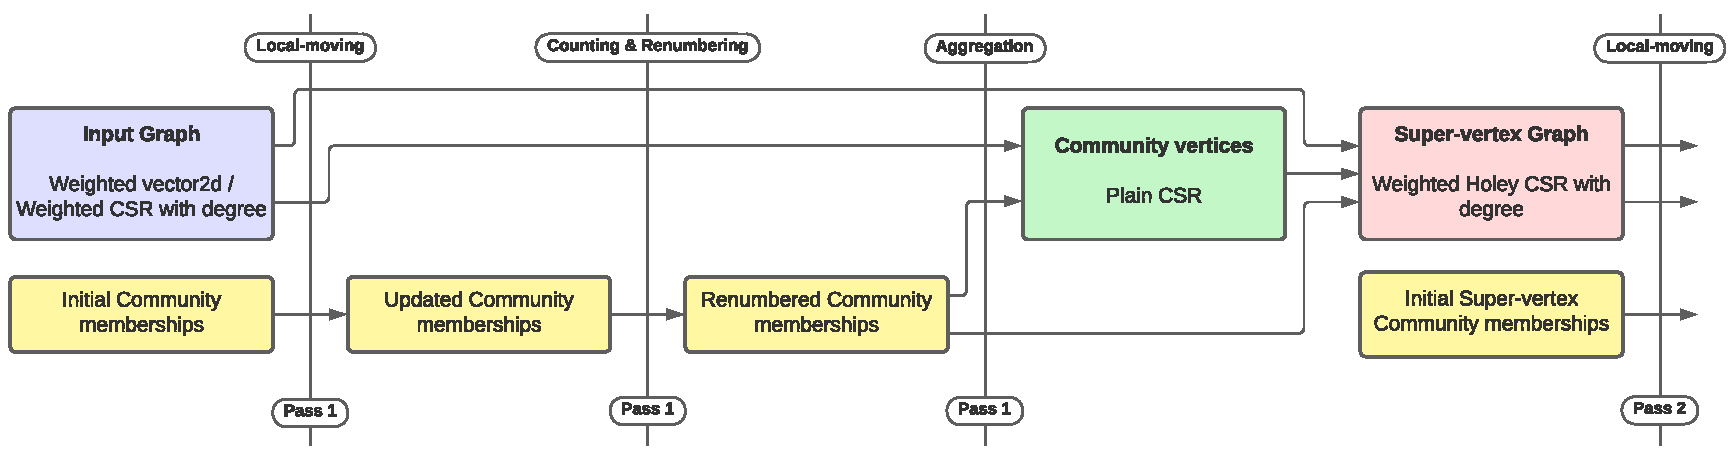
\includegraphics[width=0.98\linewidth]{out/leiden-pass.pdf}
  } \\[-2ex]
  \caption{A flow diagram illustrating the first pass of GVE-Leiden for either a Weighted 2D-vector-based or a Weighted CSR with degree-based input graph. In the local-moving phase, vertex community memberships are updated to obtain community bounds for the refinement phase, until the cumulative delta-modularity change across all vertices reaches a specified threshold. Then, in the refinement phase, the each vertex starts in a singleton community, and community memberships are updated similarly to the local-moving phase, with vertices changing communities within their bounds. These community memberships are then counted and renumbered. In the aggregation phase, community vertices in a CSR are first obtained. This is used to create the super-vertex graph stored in a Weighted Holey CSR with degree. Subsequent passes use a Weighted Holey CSR with degree and initial community memberships for super-vertices from the previous pass as input.}
  \label{fig:leiden-pass}
\end{figure*}

